%In this section we provide details of the three datasets that we evaluate in this paper, as well as the methodology used.
%\subsection{Dataset description}


%\subsubsection{Twitter example (Detection of natural disasters)}
\textcolor{red}{The scenario we have chosen to evaluate our algorithms is related to the detection of natural disasters discussed in a collection of tweets.  We used the Twitter data described in  \cite{Iman2017}, which was curated collaboratively by  four students as follows: (1) the dataset was restricted to users located within the US, (2) non-English tweets were filtered out, (3) only the tweets related to 12 natural disasters were kept -- tweets related to other natural disasters were removed. These natural disasters are temporally, and geographically disjoint -- a storm, a hurricane,  a drought, two floods, two earthquakes, two tornadoes,  and three blizzards. Finally, (4) false positive tweets were intentionally included -- tweets mentioning natural disasters specific-keywords but are not related to a particular natural disaster, e.g., \textit{\textquotedblleft I'm flooded with questions from followers\textquotedblright{}}. The final dataset contains 39,486 tweets with 5,075 marked as relevant tweets (in this context, a relevant tweet is a tweet related to a natural disaster).
}

\textcolor{red}{In addition to comparing our algorithms to the optimal solution, we also propose to use X-Means \cite{Pelleg2000} as a baseline method for clustering. X-Means is an extension of K-Means which tries to  automatically determine the number of clusters. Starting with only one cluster, the X-Means algorithm goes into action after each run of K-Means, making local decisions about which subset of the current centroids should split themselves in order to better fit the data. Also, the distance metric we have used for X-Means is a linear combination of: (i) the Euclidean distance of time, (ii) the Euclidean distance of location, and (iii) the cosine distance of the textual content. This distance metric is defined as follows:}
\begin{equation}
d(i,j) = \alpha\times\textrm{[time dist.]}+\beta\times \textrm{[location dist.]}+\gamma\times \textrm{[text cosine dist.]}
\end{equation}
\textcolor{red}{\noindent where $\alpha$, $\beta$, and $\gamma$ are weights that sum to 1, set all to 1 in the off-line evaluation and set respectively to 0.1, 0.8,  and 0.1 in the user study -- values manually tuned by our four students. Finally, we used EF1 to rank clusters returned by X-Means. }

%We assume having an agent monitoring tweets, a topical tweets classifier (e.g., \cite{Iman2017}), and a display showing the locations of the tweets (See Figure \ref{Fig:TwitterData}).  We used the  2.5 TB of Twitter data described in  \cite{Iman2017}, for which we restricted our analysis to the 9M tweets of January 2014.





%\begin{figure}[t]
%\begin{centering}
%\subfigure[Twitter Networks.]{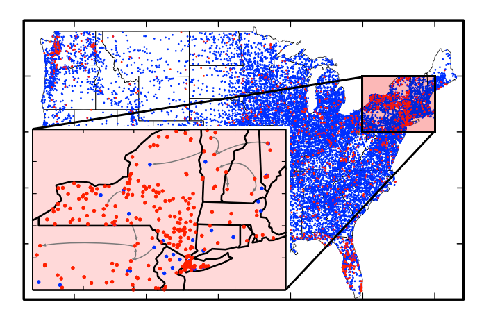
\includegraphics[width=2.8cm]{imgs/twitter_example_3}\label{Fig:TwitterData}}\subfigure[Enron Networks.]{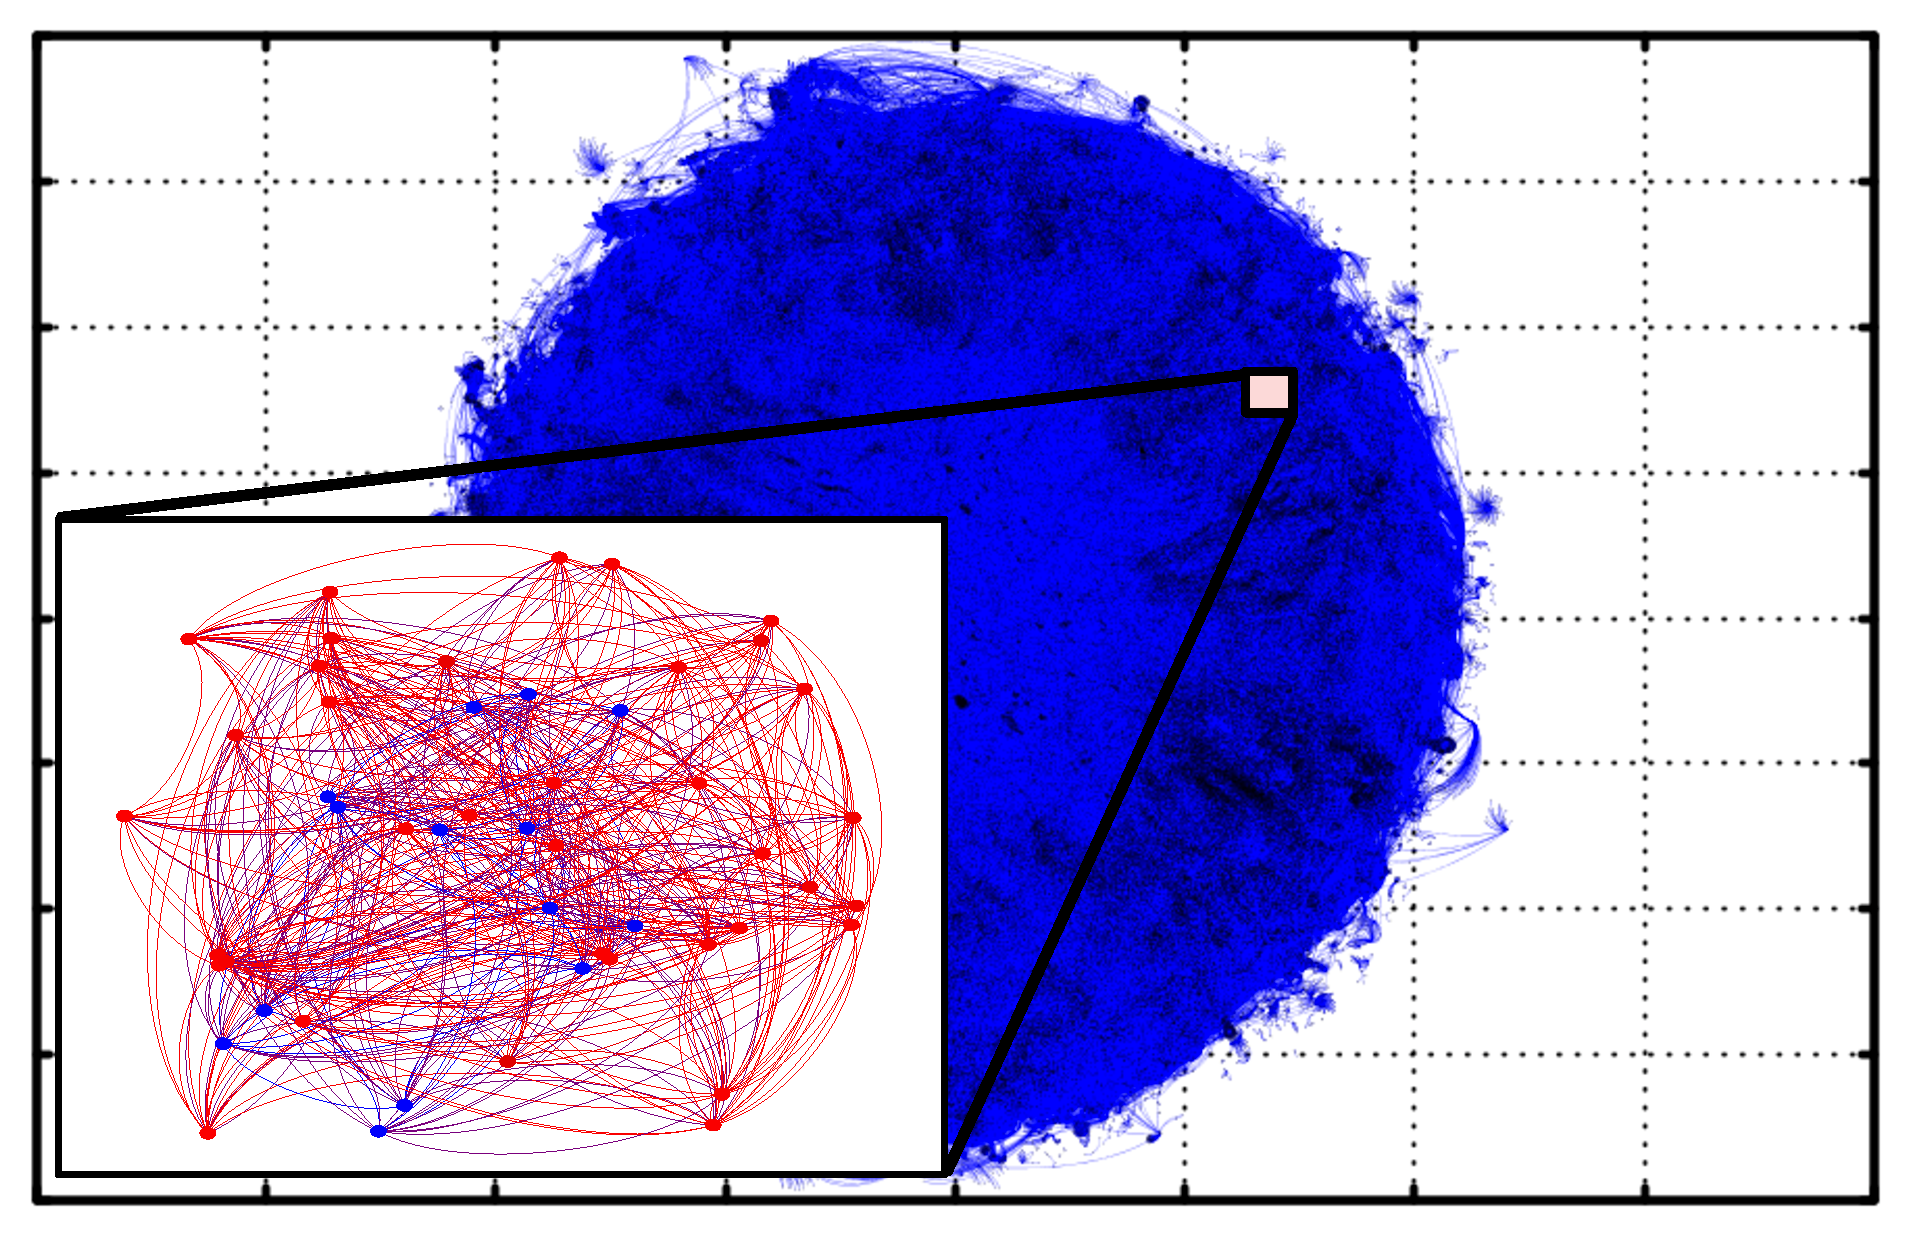
\includegraphics[width=2.8cm]{imgs/enron_net_4}\label{Fig:EnronData}}\subfigure[Reddit Networks.]{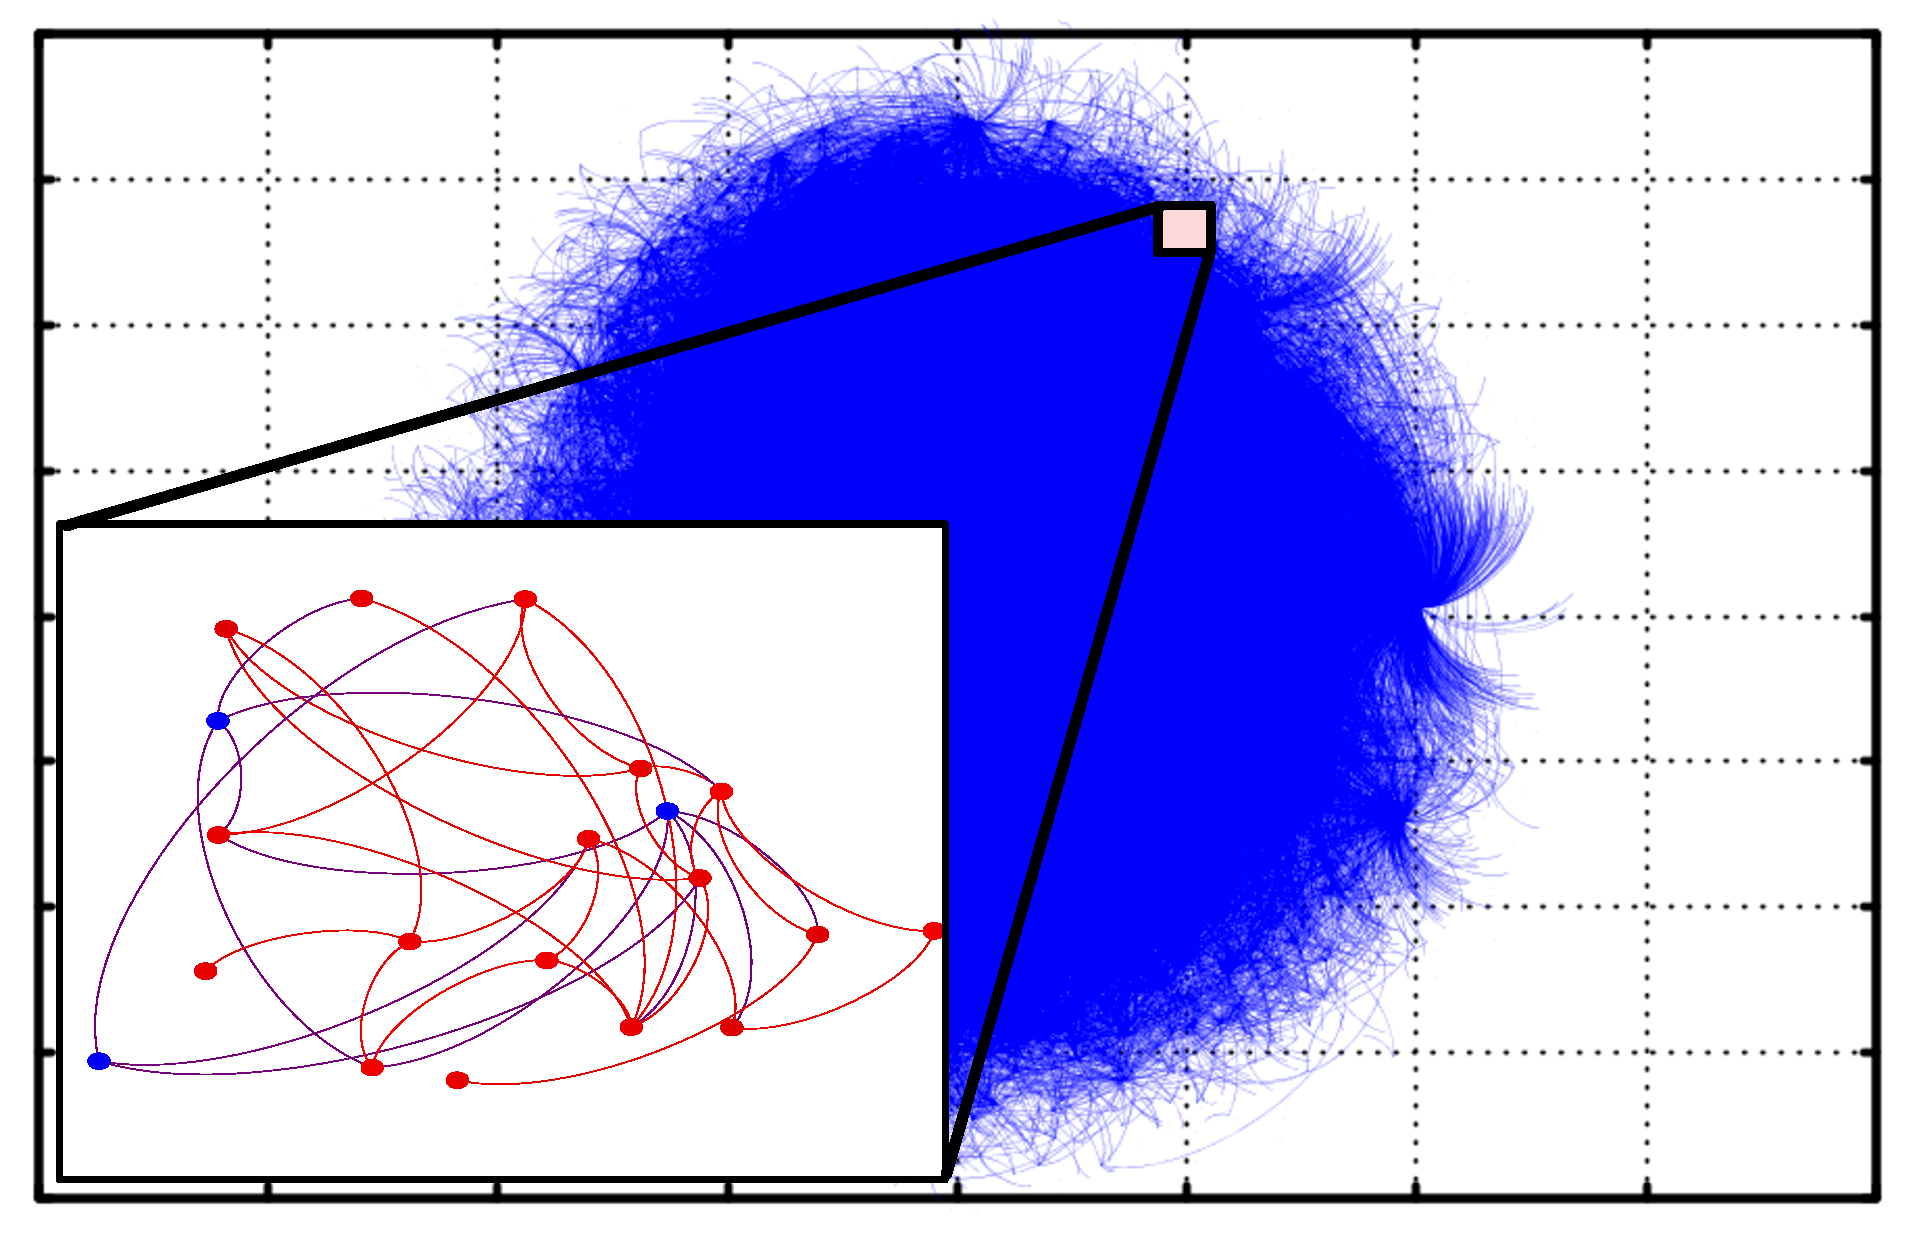
\includegraphics[width=2.8cm]{imgs/srforum3}\label{Fig:RedditData}}
%\par\end{centering}
%\caption{Layouts used for the different datasets.}
%\end{figure}





